\documentclass{beamer}
\usepackage[utf8x]{inputenc}
\usepackage[T1]{fontenc}
\usepackage{booktabs,multicol,lmodern,amsmath}
% \usetheme{ICM}
\usetheme{Berlin}
\xdefinecolor{icmgreen}{rgb}{0,0.55,0.46}
\usecolortheme[named=icmgreen]{structure}
\newcommand{\email}[1]{\textcolor{blue}{\textsf{#1}}}

\title{Dynamika sieci aliansów strategicznych pomiędzy firmami}

\subtitle{Umiędzynarodowienie i zróżnicowanie technologiczne}

\author[Michał Bojanowski <m.bojanowski@uw.edu.pl>]{Michał Bojanowski\\ \email{m.bojanowski@uw.edu.pl}}

\date{12 marca, 2015}

\institute{ICM UW}


\renewcommand{\emph}[1]{\textbf{#1}}


\begin{document}


\begin{frame}
	\titlepage
\end{frame}

\section{Wprowadzenie}

\begin{frame}{Alianse strategiczne między firmami}
	Alianse strategiczne:
	\begin{itemize}
		\item Dobrowolna umowa o długotrwałej współpracy.
		\item Wiele typów/powodów tworzenia aliansów, m.in.: R\&D, licencyjne, produkcyjne.
		\item Transakcja pomiędzy hierarchią a wolnym rynkiem (Powell, 1990).
		\item Alians jako narzędzie zarządzania współzależnością
			(\textit{interdependence}) pomiędzy firmami (Gulati \& Gargiulo, 1999).
	\end{itemize}
\end{frame}

\begin{frame}{Alianse R\&D 1989--2002}
	\centering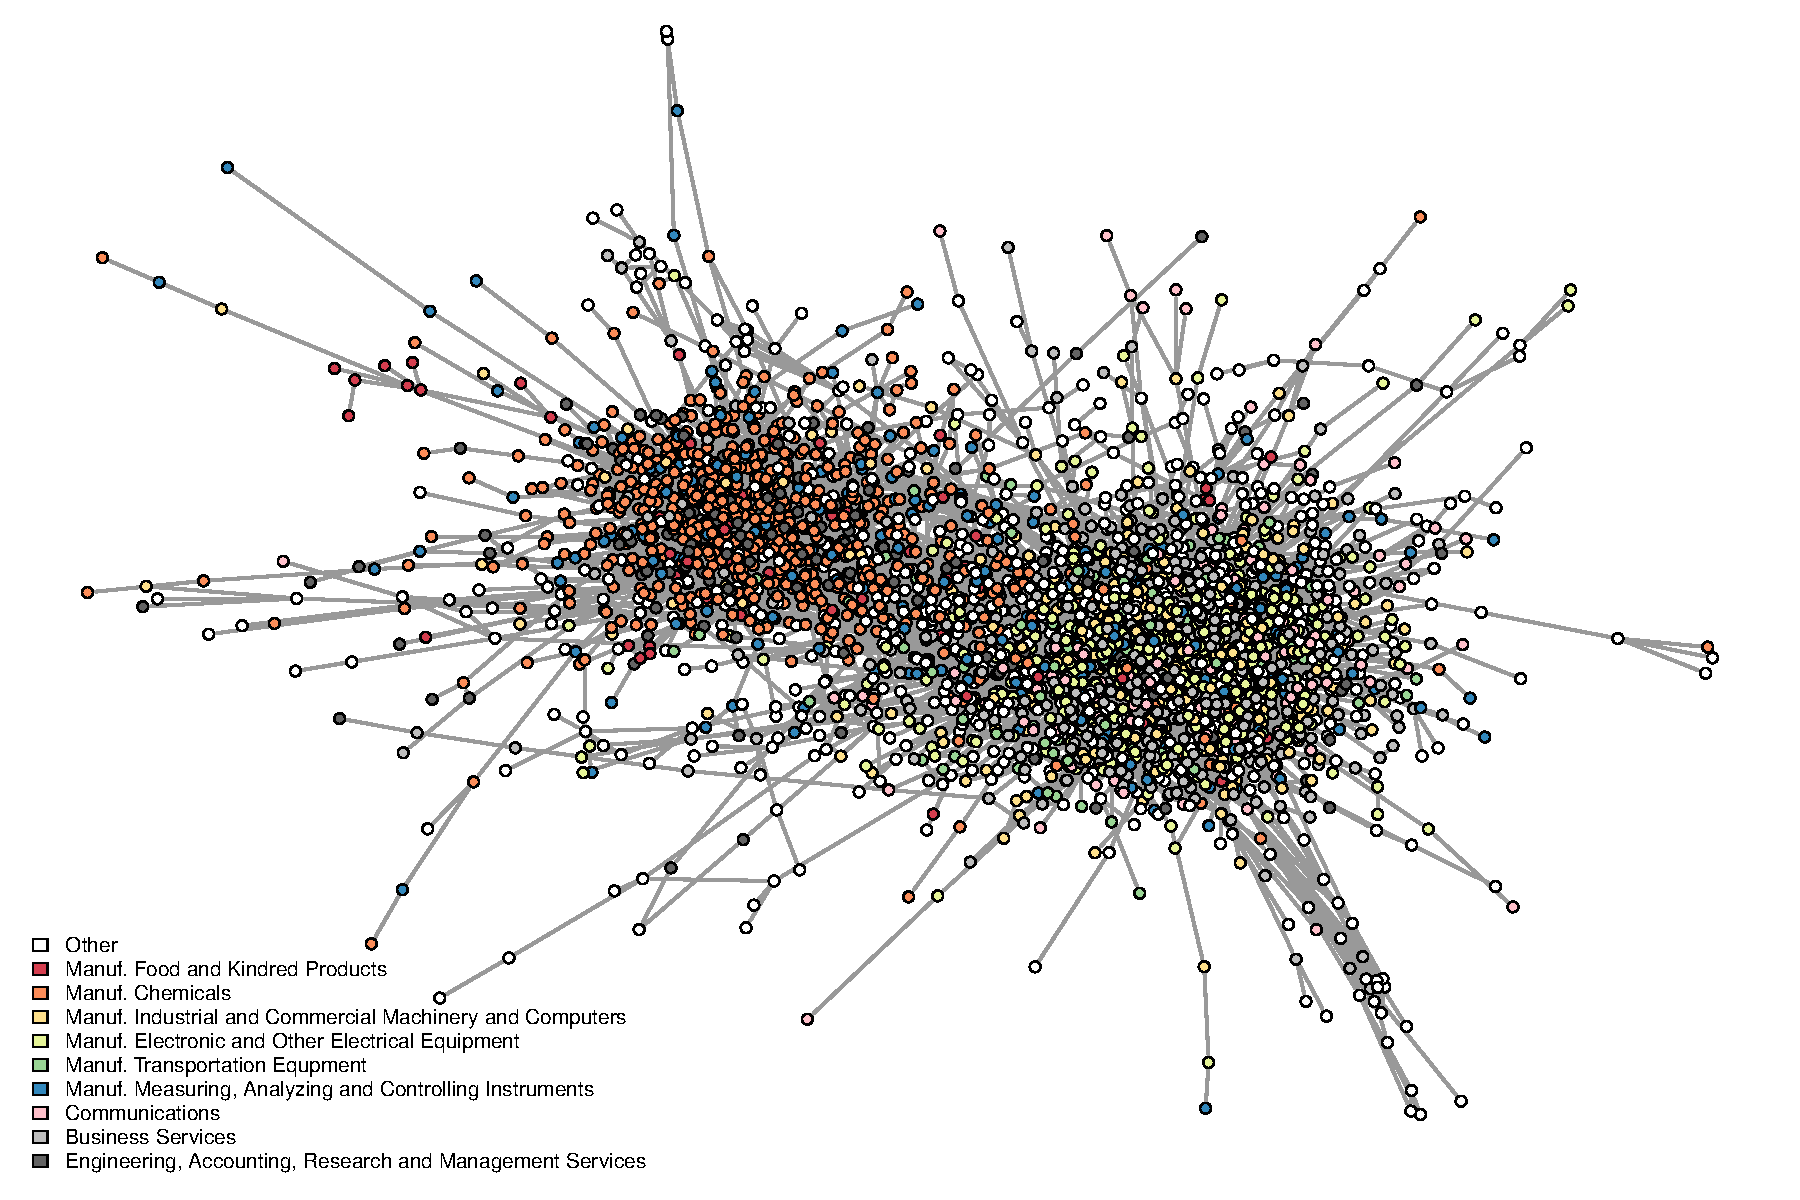
\includegraphics[width=\textwidth]{thomson-sec2}

	\begin{footnotesize}
		Dane: Thomson SDC Platinum
	\end{footnotesize}
\end{frame}



\begin{frame}{Dwa pytania badawcze}
	\begin{enumerate}
		\item Czy globalna sieć aliansów stała się bardziej czy mniej zintegrowana
			w latach 1989--2002?
		\item Czy strukturę sieci aliansów można (częściowo) wyjaśnić
			różnorodnością technologii i strukturą gospodarki?
	\end{enumerate}
\end{frame}


\section{Integracja międzynarodowa}

\begin{frame}
	\begin{center}
		\begin{Huge}
		Integracja w międzynarodowej sieci aliansów
		\end{Huge}
	\end{center}
\end{frame}

\begin{frame}
	\begin{itemize}
		\item Czy globalna sieć aliansów stała się bardziej czy mniej zintegrowana
			w latach 1989--2002?
	\end{itemize}

	Dwie sprzeczne hipotezy:
	\begin{enumerate}
		\item Aliansów międzynarodowych spodziewamy się coraz \emph{więcej}.
			\begin{footnotesize}
				Liberalizacja międzynarodowego prawa własności sprawiła, że
				procesy produkcyjne są rozproszone po całym świecie. Współpraca
				międzynarodowa jest konieczna by tymi procesami zarządzać.
				(Duysters \& Hagedoorn, 1996; Narula 1996).
			\end{footnotesize}

		\item Aliansów międzynarodowych spodziewamy się coraz \emph{mniej}.
			\begin{footnotesize}
				Strategiczne alianse międzynarodowe to tylko środek zastępczy omijający
				międzynarodowe bariery utrudniające wykup/przejęcia.  Gdy bariery
				znikną, firmy zastąpią alianse ponadnarodowe bezpośrednim inwestowaniem lub
				wykupywaniem spółek w innych krajach. (Contractor, 1990; Desai et al., 2004).
			\end{footnotesize}
	\end{enumerate}
	Homofilia wg przynależności państwowej firm.
\end{frame}


\begin{frame}{Preferencje vs aktywność vs podaż partnerów}
	Nie jesteśmy pierwsi!
	\begin{itemize}
		\item Hagedoorn (1996, 2002): odsetek aliansów międzynarodowych maleje więc
			współpraca międzynarodowa mniej istotna dla firm.
	\end{itemize}

	\emph{Niekoniecznie!} Możliwe alternatywne wyjaśnienia:
	\begin{footnotesize}
		\begin{enumerate}
			\item Firmy w państwie X są mniej zainteresowane partnerstwami z firmami z
				innych krajów.
			\item Wzrosła liczba firm w państwie X co sprawia, że jest więcej okazji
				nawiązania współpracy wewnętrznej (homofilia).
			\item Firmy w państwie X nawiązują mniej aliansów bez względu na "narodowość"
				partnera.
		\end{enumerate}
	\end{footnotesize}
	Aby wykluczyć (2) i (3) należy
	\begin{itemize}
		\item Wziąć pod uwagę strukturę populacji firm: dodatkowe dane WDI.
		\item Użyć odpowiedniej miary: wariant indeksu Colemana.
	\end{itemize}
\end{frame}


\begin{frame}{Wyniki i niuanse}
	\centering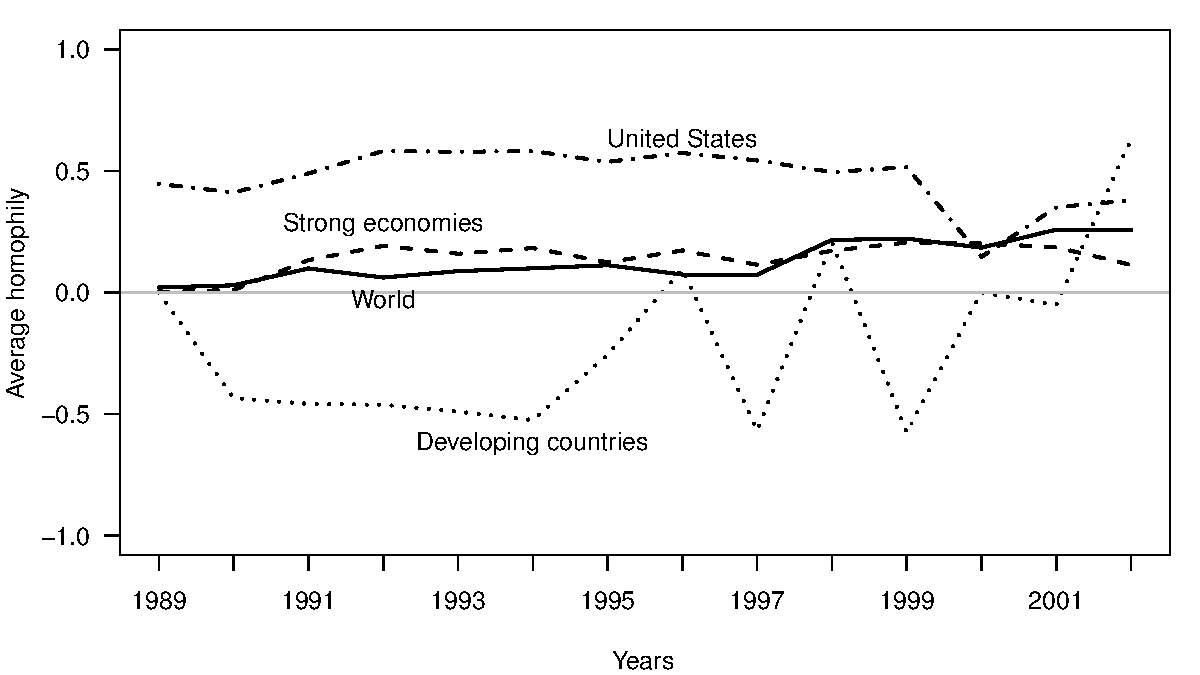
\includegraphics[width=\textwidth]{figure2}

	Dane: Thomson SDC Platinum + WDI.
	8155 aliansów R\&D, 3555 uczestników spośród 31671 firm.
\end{frame}











\section{Technologia i struktura gospodarki}

\begin{frame}
	\begin{center}
		\begin{Huge}
			Zróżnicowanie technologiczne tworzenie się aliansów
		\end{Huge}
	\end{center}
\end{frame}

\begin{frame}{Współzależności jako efekt struktury gospodarki}

	\begin{itemize}
		\item Firma to jednostka organizacyjna przetwarzająca czynniki produkcji
			(inputs) w produkty (outputs) sprzedawane na rynku (inne firmy lub
			indywidualna konsumpcja).

		\item Technologia to mapowanie pomiędzy czynnikami a produktami.

		\item Podstawowym mechanizmem generującym złożone współzależności między
			firmami są \emph{łańcuchy wartości} (\textit{value chain}).

		\item Struktura łańcuchów wartości wynika z podaży produktów i popytu na
			czynniki produkcji.
	\end{itemize}

	\begin{block}{Pytanie}
		Jakie formy współzależności sprzyjają nawiązywaniu aliansów?
	\end{block}
\end{frame}


\begin{frame}{Formy współzależności}
	Możemy wyróżnić następujące formy współzależności pomiędzy sektorami $A$ i
	$B$ gospodarki:

	\bigskip

	Bezpośrednia:
	\begin{description}
		\item[współzależność wertykalna] $A$ jest istotnym dostawcą dla $B$ lub vice versa.
	\end{description}

	Pośrednie:
	\begin{description}
		\item[komplementarność] Produkty $A$ i $B$ są ważnymi czynnikami dla $C$.
		\item[podobieństwo struktury czynników] $A$ i $B$ potrzebują produktów z $C$.
		\end{description}
\end{frame}




\begin{frame}{Struktura gospodarki USA}
	\centering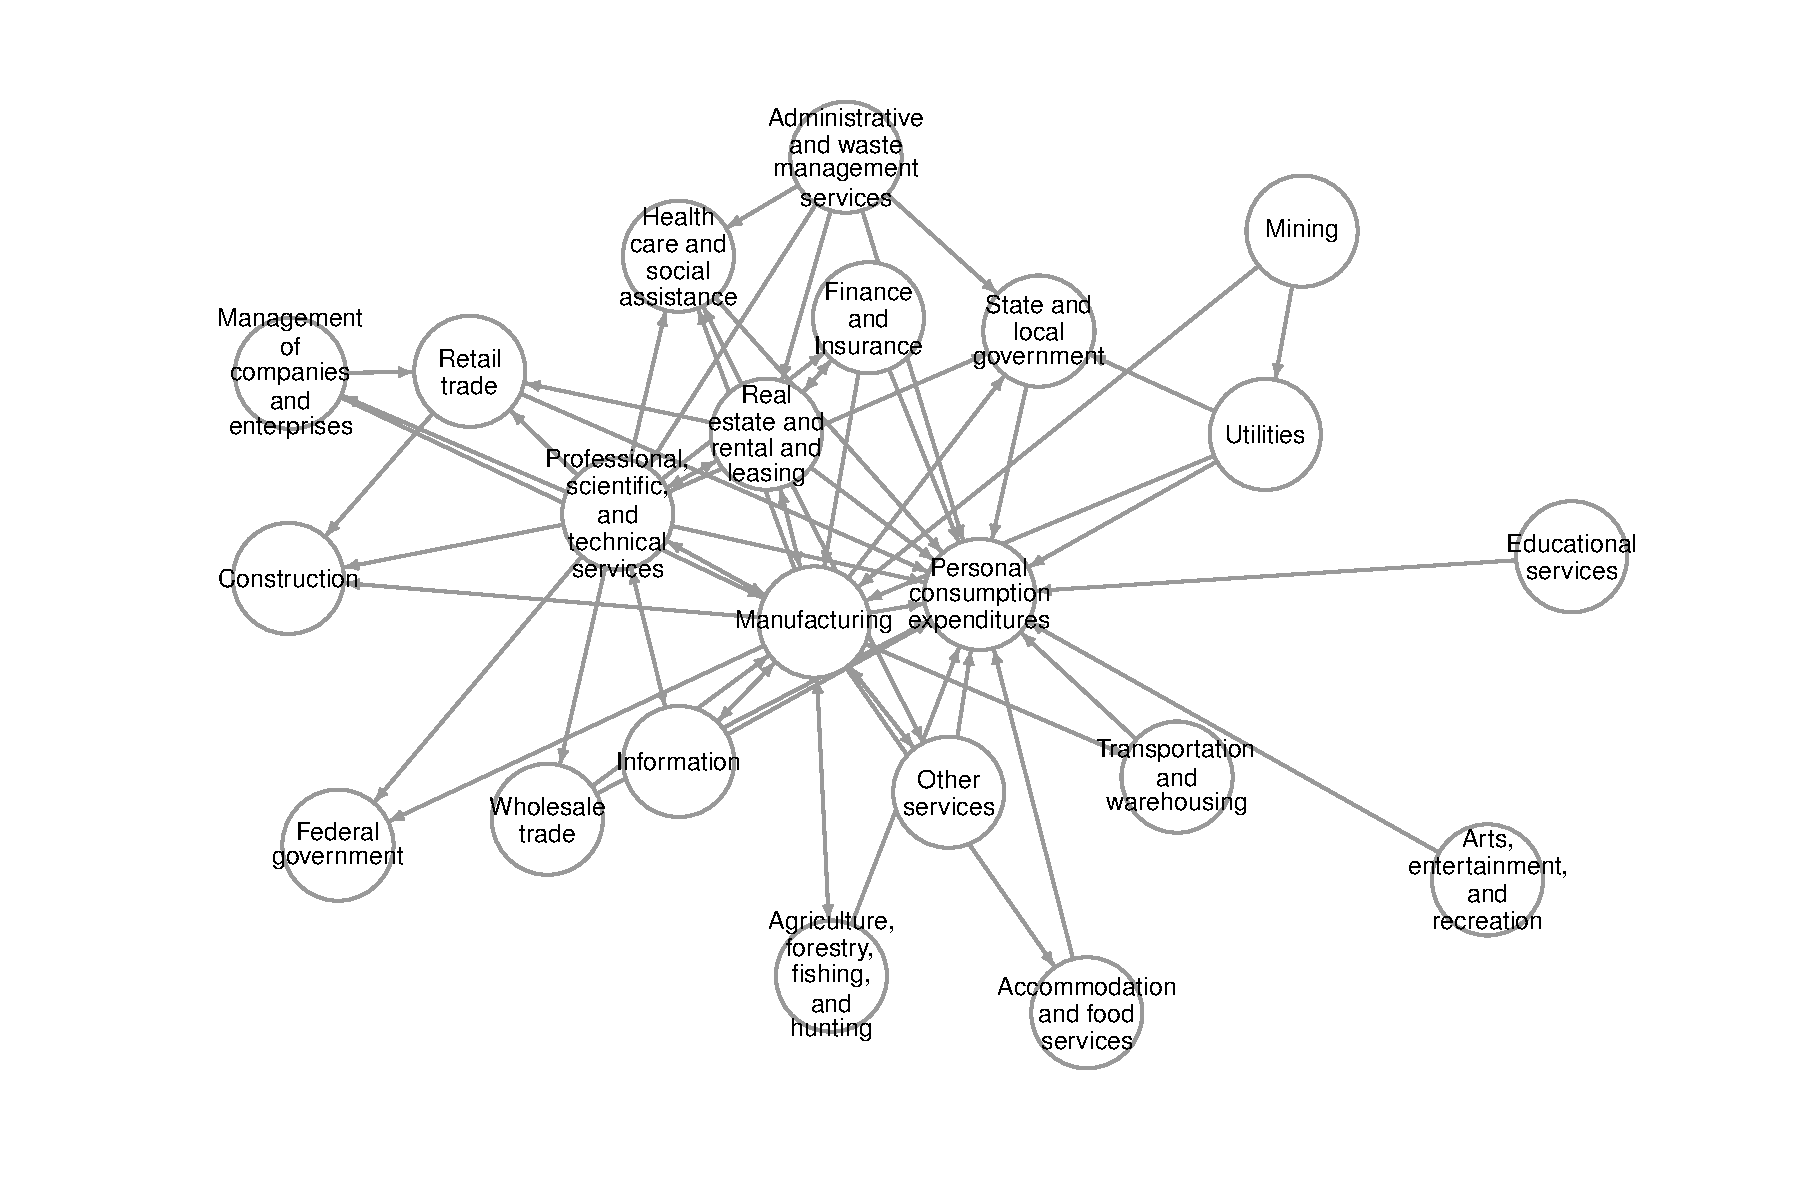
\includegraphics[width=\textwidth]{ioflowtop}

	Dane: US Bureau of Economic Analysis 1998--2005.
\end{frame}




\begin{frame}{Dane i model}
	Dane:
	\begin{itemize}
		\item Thomson SDC (alianse), BEA (input-output).
		\item 17865 aliansów pomiędzy 29879 firmami w USA.
		\item Tylko alianse między-sektorowe.
	\end{itemize}

	Model:
	\begin{equation*}
		\log \left( \frac{p_{ij}}{1-p_{ij}} \right) =
		\alpha + \sum_{k=2}^{M=20} \beta_k D_k +
		\beta_V V_{ij} + \beta_C C_{ij} + \beta_I I_{ij} +
		\beta_{VI} V_{ij} I_{ij}
		\quad (i \neq j)
	\end{equation*}
	Przewidujemy szanse zawiązania aliansów pomiędzy firmami z sektorów $i$ i $j$
	za pomocą trzech typów współzależności ($V_{ij}$, $C_{ij}$, $I_{ij}$) kontrolując
	zróżnicowanie aktywności w formowaniu aliansów pomiędzy sektorami ($D_k$).
\end{frame}


\begin{frame}{Wyniki}
	\begin{itemize}
		\item Silna współzależność wertykalna = alianse prawie 20-krotnie częstsze.
		\item Brak efektu komplementarności.
		\item Negatywny efekt podobieństwa struktury czynników.
			\begin{footnotesize}
				\begin{itemize}
					\item Istotny statystycznie, ale mało istotny substantywnie
					\item Konkurencja o dostawców?
				\end{itemize}
			\end{footnotesize}
	\end{itemize}
\end{frame}



\begin{frame}
	\begin{center}
		\begin{Huge}
			Dziękuję!
		\end{Huge}
	\end{center}
\end{frame}


\begin{frame}{Dziękuję!}
	\begin{footnotesize}
		Po więcej szczegółów odsyłam do:
		\begin{itemize}
			\item Bojanowski, Corten, Westbrock (2011) "The Structure and Dynamics of
				Global Network of Inter-firm R\&D Partnerships 1989--2002.
				\textit{Journal of Technology Transfer} 37:6, 967--987.
			\item Bojanowski (2011) "Industrial Structure and Inter-firm Collaboration",
				ISCORE Discussion Paper 279.
			\item Bojanowski (2012) \textit{Essays on Social Network Formation in Heterogeneous Populations},
				Utrecht: ICS.
			\item Bojanowski, Corten (2014) "Measuring Segregation in Social Networks",
				\textit{Social Networks} 39, 14--32.
		\end{itemize}
	\end{footnotesize}
\end{frame}

\end{document}
